\chapter{Referencial Teórico}\label{cap:referencial}

A seguir é apresentado o referencial teórico que fundamenta o desenvolvimento de uma abordagem de versionamento. Inicialmente, são discutidos os conceitos relacionados aos sistemas de controle de versões, com ênfase no funcionamento e nas características do sistema Git e de suas extensões voltadas ao gerenciamento de arquivos de grande porte. Em seguida, são apresentados diferentes modelos de escrita utilizados em sistemas de arquivos modernos, abordando as estratégias empregadas para registrar modificações em dados e preservar versões anteriores. Posteriormente, são discutidos sistemas de arquivos que utilizam essas abordagens, bem como aspectos relacionados ao tratamento de arquivos binários em processos de armazenamento e versionamento. Por fim, é apresentado o objeto de teste adotado neste trabalho, um tipo de arquivo binário utilizado na modelagem tridimensional que apresenta características relevantes para os processos de versionamento, sendo descrita sua estrutura e funcionamento.

\section{Sistema de controle de versões}

Um sistema de controle de versões é uma ferramenta utilizada durante o fluxo de trabalho de desenvolvimento para gerenciar alterações em arquivos ao longo do tempo. Esse controle permite rastrear o histórico de evolução de um projeto e possibilita a colaboração entre múltiplos desenvolvedores simultaneamente. Por meio de mecanismos como registro de alterações, revisão de código, gerenciamento de versões e ferramentas de colaboração, esses sistemas organizam o desenvolvimento de forma estruturada, garantindo a integridade do código e a coordenação entre diferentes contribuições, além de permitir o gerenciamento das diferentes versões de um sistema ou aplicação \cite{Spinellis2005}.

O uso de sistemas de controle de versão é uma prática fundamental para o desenvolvimento profissional de \textit{software}, pode-se comparar a prática de usá-los com a importância do uso de editores de texto ou compiladores. Implementar o controle de versões a nível empresarial pode envolver custos iniciais e uma curva de aprendizado, mas a sua ausência compromete a organização e a evolução de projetos de produção \cite{Spinellis2005}.

Um sistema de controle de versões atua, na prática, como uma máquina do tempo para cada projeto, permitindo que a equipe de desenvolvimento gerencie o histórico de alterações de forma ampla e segura. Em cenários de trabalho em equipe, a principal vantagem é evitar que os desenvolvedores sobrescrevam o trabalho alheio \cite{Spinellis2005}. Como exemplos de sistemas de controle de versão tem-se o Subversion e o Git. 

\subsection{O Sistema de Controle de Versão Git}

O Git é um sistema de controle de versão distribuído amplamente adotado devido à sua rapidez e eficiência no gerenciamento de projetos de \textit{software}, em contraste com os modelos centralizados. O Git permite que cada colaborador possua um repositório privado completo em seu ambiente de trabalho. Essa arquitetura descentralizada garante que os desenvolvedores possam realizar \textit{commits}, editar históricos e criar ramificações de forma independente, sem afetar o trabalho de terceiros ou depender de uma conexão constante com o servidor principal \cite{Cunha2018}.

No Git, o estado atual do trabalho é monitorado por um ponteiro chamado \textit{HEAD}, que indica a ramificação e o comando mais recente realizado. Todas as ações executadas localmente são registradas automaticamente em um arquivo de registro, que funciona como um rastro histórico das ações realizadas no repositório. Para consolidar o trabalho individual no repositório principal, os desenvolvedores utilizam mecanismos de integração, sendo o \textit{merge} o mais tradicional por registrar explicitamente a união de duas linhagens de código em um novo \textit{commit} \cite{Cunha2018}.

Apesar de sua eficiência em relação ao código-fonte, o Git enfrenta gargalos significativos ao lidar com conteúdo binário e arquivos de grande porte, uma vez que o sistema foi projetado para armazenar o histórico completo de cada arquivo. Contudo,  arquivos binários não permitem operações de comparação diferencial ou compressão de forma eficaz, como ocorre em arquivos de texto. Consequentemente, qualquer pequena alteração em um binário resulta no armazenamento de uma nova cópia integral do arquivo, causando uma rápida e ineficiente expansão do tamanho do repositório. Essa limitação motiva o uso de extensões e de abordagens alternativas de armazenamento que operem de forma mais granular \cite{Chen2025}.

Entre essas soluções, tem-se o \gls{gitlfs}, uma extensão amplamente adotada na indústria de software para lidar com arquivos pesados, que, ao serem versionados, normalmente vão inflar o armazenamento do repositório tradicional do Git \cite{Chen2025}. O \gls{gitlfs} se baseia na substituição de arquivos binários relativamente grandes por arquivos de ponteiro textuais dentro do repositório principal. Esses ponteiros servem como referências para o conteúdo real do arquivo que está em um ambiente externo, um servidor \gls{lfs} especializado. Com isso, o repositório Git mantém apenas metadados sobre cada arquivo, como o identificador criptográfico, \textit{hash}, e o tamanho do arquivo. Os dados do binário são recuperados apenas durante operações de sincronização ou recuperação de versões do repositório.

Essa abordagem permite reduzir significativamente o crescimento do repositório principal e otimizar processos como clonagem e sincronização de projetos. No entanto, ao deslocar o armazenamento dos arquivos para uma infraestrutura externa, o \gls{gitlfs} introduz novas camadas de complexidade relacionadas à gestão de recursos, ao desempenho da infraestrutura e à segurança do sistema \cite{Chen2025}.

\section{Modelos de escrita para sistemas de arquivos}

Existem duas políticas fundamentais utilizadas para atualizar blocos de dados em dispositivos de armazenamento: o modelo de sobrescrita direta, conhecido como \gls{uip}, e abordagens que evitam a modificação direta do conteúdo previamente gravado. No modelo \gls{uip}, o bloco de dados é inicialmente carregado para a memória, modificado e posteriormente gravado novamente no disco exatamente na mesma posição física, substituindo o conteúdo anterior. Em contrapartida, arquiteturas mais recentes adotam estratégias nas quais os dados modificados são registrados em novas regiões do dispositivo de armazenamento, preservando a versão anterior do bloco \cite{Chen2014}.

Essas abordagens de escrita são amplamente utilizadas em diferentes áreas da computação. Além de sistemas de arquivos modernos, neles os mecanismos também são empregados em sistemas de gerenciamento de bancos de dados para controle transacional, na gerência de memória virtual para compartilhamento eficiente de páginas entre processos e em ambientes de virtualização utilizados na criação de discos virtuais. O objetivo principal dessas estratégias é aumentar a confiabilidade do sistema e facilitar a manutenção da consistência dos dados, permitindo a recuperação em situações de falha e viabilizando recursos como \textit{snapshots} e clonagem de estados do sistema. Nas subseções seguintes são apresentados os principais modelos utilizados para implementar essas estratégias de atualização de dados \cite{Xiao2009}, as quais são utilizadas nos sistemas de arquivos modernos, como \gls{btrfs} e \gls{zfs}.

\subsection{\textit{Copy-On-Write} e \textit{Redirect-On-Write}}

O modelo \gls{cow} possui como princípio fundamental evitar a sobrescrita direta de dados já existentes, garantindo que versões anteriores possam ser preservadas. Enquanto múltiplos processos necessitam apenas realizar operações de leitura sobre um determinado dado, eles podem compartilhar ponteiros para a mesma estrutura em disco. Entretanto, quando ocorre a primeira tentativa de escrita em um bloco após a criação de um \textit{snapshot}, o sistema executa uma sequência de operações: inicialmente, o bloco original é lido; em seguida, uma cópia desse bloco é registrada no volume associado ao \textit{snapshot}; por fim, a nova versão modificada do bloco é gravada na estrutura ativa do sistema de arquivos \cite{Xiao2009}.

Esse mecanismo pode ser comparado, de forma análoga, à aquisição de um imóvel: embora exista um custo inicial mais elevado associado à sua obtenção, as operações subsequentes de uso e manutenção tornam-se mais diretas e eficientes. De maneira semelhante, o \gls{cow} introduz um custo adicional no momento da primeira modificação de um bloco, mas permite otimizações significativas nas operações posteriores \cite{Peterson2005}.

Para ilustrar o funcionamento desse modelo, considera-se um arquivo binário dividido em cinco blocos de dados. Na Figura~\ref{fig:cow-inicial}, observa-se o estado inicial do arquivo, no qual cada bloco é referenciado por ponteiros armazenados no sistema de arquivos \cite{Xiao2009}.

\begin{figure}[htb]
  \centering
  \caption{\label{fig:cow-inicial}Estado inicial do arquivo binário dividido em blocos}
  \fbox{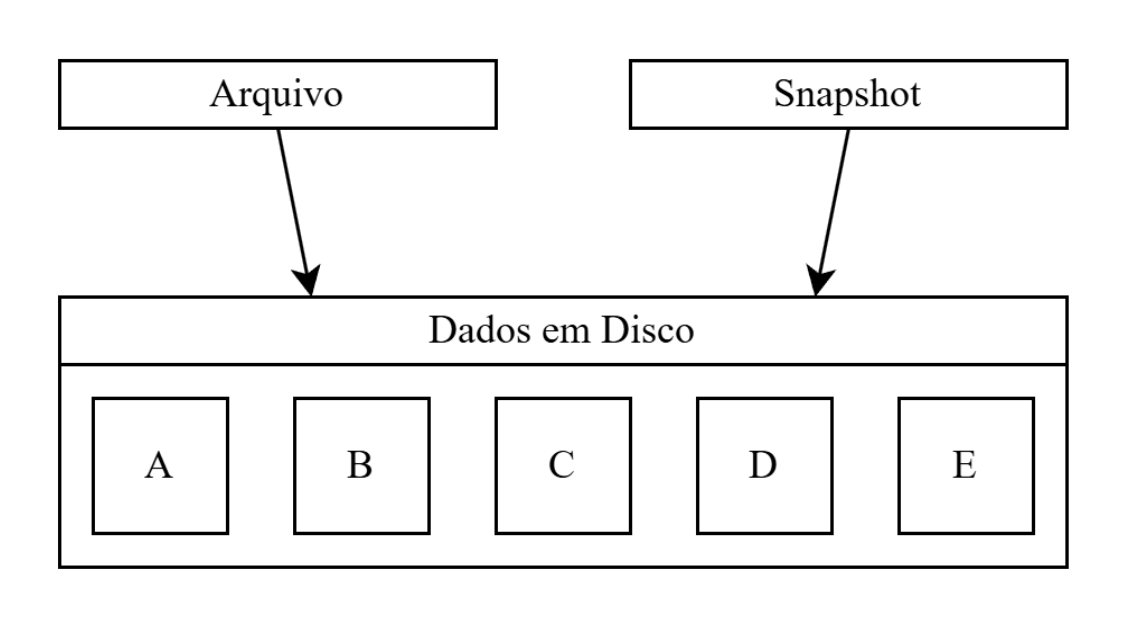
\includegraphics[width=0.8\textwidth]{figuras/cow-estado-inicial.png}}
  \fonte{Autoria própria}
\end{figure}

Conforme demonstrado na Figura~\ref{fig:cow-final}, quando ocorre uma modificação em um dos blocos do arquivo, o mecanismo \gls{cow} evita a sobrescrita direta do bloco original. Em vez disso, um novo bloco é alocado no disco para armazenar a versão modificada dos dados, enquanto o bloco original permanece preservado. Os ponteiros do sistema são então atualizados para referenciar o novo bloco, mantendo intacta a versão anterior dos dados. Olhando o \textit{snapshot} ilustrado na Figura~\ref{fig:cow-final}, observa-se que apenas o bloco C foi modificado após a criação da imagem do sistema. Como resultado, o mecanismo \gls{cow} cria um novo bloco C$'$, para armazenar a versão atualizada dos dados, enquanto o bloco C original permanece preservado e continua sendo referenciado pelo \textit{snapshot}. Os demais blocos (A, B, D e E) não sofreram alterações e, portanto, permanecem compartilhados entre o estado atual do arquivo e o \textit{snapshot} \cite{Xiao2009}.

\begin{figure}[htb]
  \centering
  \caption{\label{fig:cow-final}Disco após as mudanças no arquivo}
  \fbox{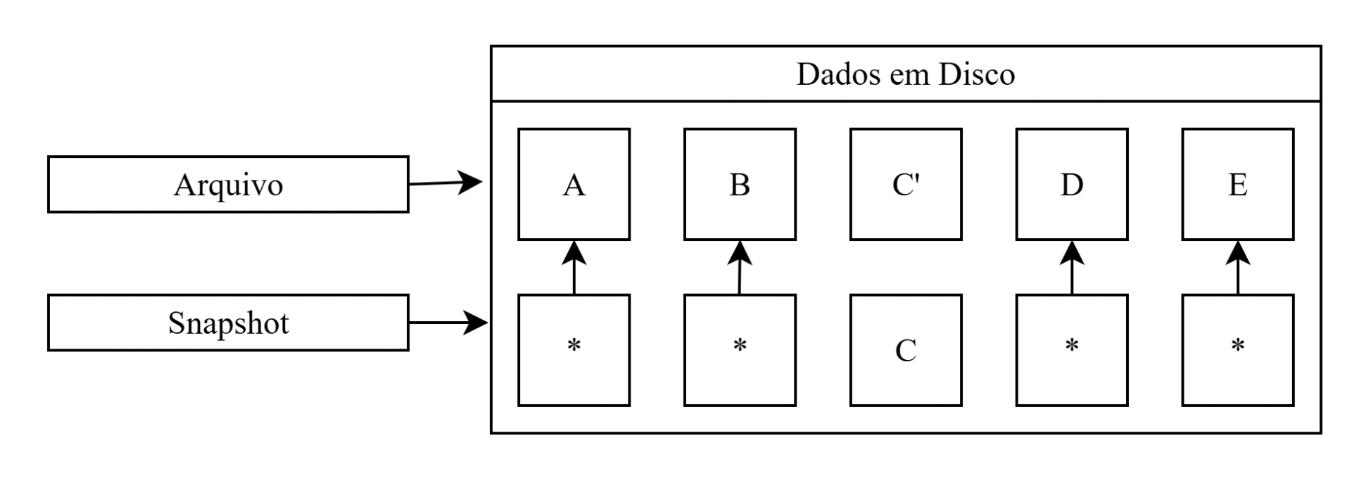
\includegraphics[width=0.8\textwidth]{figuras/cow-estado-final.png}}
  \fonte{Autoria própria}
\end{figure}

Esse comportamento permite a criação eficiente de versões e \textit{snapshots} do arquivo, uma vez que apenas os blocos efetivamente modificados precisam ser armazenados novamente, reduzindo o consumo de espaço e possibilitando a recuperação de estados anteriores do sistema \cite{Xiao2009}.

No mecanismo \gls{row} quando ocorre uma modificação em um bloco de dados que já está sendo referenciado por um \textit{snapshot}, o sistema não realiza a cópia prévia do bloco original. Em vez disso, o bloco existente permanece inalterado em sua posição no disco, preservando a versão anterior dos dados. A nova escrita é então direcionada diretamente para um novo bloco, localizado em outra região do armazenamento. Dessa forma, o \textit{snapshot} continua apontando para o bloco original, enquanto a versão atualizada do arquivo passa a referenciar o novo bloco que contém as modificações \cite{Xiao2009}.

Essa abordagem reduz a sobrecarga inicial presente no modelo \gls{cow}, pois elimina a necessidade de ler e copiar o bloco original antes de registrar a nova versão. Como resultado, o \gls{row} tende a apresentar melhor desempenho em cenários caracterizados por operações intensivas de escrita, nos quais a penalidade da primeira modificação poderia impactar significativamente a performance do sistema \cite{Xiao2009}.

Por outro lado, o uso do \gls{row} pode introduzir maior complexidade nas operações de leitura. Como os dados modificados são gravados em novos blocos distribuídos pelo disco, a estrutura lógica de um arquivo pode tornar-se mais fragmentada ao longo do tempo. Dessa forma, para reconstruir o estado atual de um arquivo, o sistema pode precisar acessar blocos localizados em diferentes regiões do armazenamento, o que pode aumentar o custo das operações de leitura e gerenciamento de dados \cite{Xiao2009}.

Nesse sentido, enquanto o \gls{cow} prioriza a preservação das versões anteriores por meio da cópia explícita dos blocos modificados, o \gls{row} busca otimizar o desempenho das operações de escrita ao redirecionar diretamente as modificações para novos blocos, mantendo intactos os dados previamente armazenados \cite{Xiao2009}.

\section{Sistema de arquivos modernos usando \gls{cow}}

Os sistemas de arquivos modernos, como \gls{btrfs} e \gls{zfs}, adotam o modelo \textit{Copy-on-Write} para organização e persistência de dados, utilizando a escrita em novos blocos e a atualização de ponteiros como estratégia para manter a consistência do sistema. Essa abordagem permite maior confiabilidade diante de falhas e viabiliza funcionalidades como \textit{snapshots} e versionamento eficiente, ao mesmo tempo em que introduz implicações estruturais e de desempenho que serão discutidas a seguir a partir da análise desses sistemas \cite{Benites2025}.

\subsection{\textit{B-tree File System}}

O \gls{btrfs} é um sistema de arquivos moderno desenvolvido para o ecossistema Linux com o objetivo de oferecer maior escalabilidade, integridade de dados e recursos avançados de gerenciamento de armazenamento. Sua arquitetura foi projetada para operar de forma integrada com o modelo \gls{cow}, permitindo que modificações em dados e metadados sejam registradas em novos blocos, preservando as versões anteriores e garantindo maior consistência em cenários de falha \cite{Benites2025}.

Internamente, o sistema de arquivos \gls{btrfs} organiza o estado persistente do sistema por meio de múltiplas árvores-B, responsáveis por estruturar diferentes tipos de informações, como arquivos, metadados, extensões e verificações de integridade. Essa estrutura utiliza uma variação otimizada para ambientes \gls{cow}, permitindo que alterações em nós da árvore sejam registradas sem a necessidade de reconstrução completa da estrutura. Além disso, o sistema emprega o conceito de \textit{extents}, que representam sequências contíguas de blocos em disco, favorecendo operações de leitura e escrita sequenciais e contribuindo para um uso mais eficiente do espaço de armazenamento \cite{Benites2025}.

Uma das características mais relevantes do \gls{btrfs} é o suporte nativo a \textit{snapshots} e clones, possibilitado pela própria natureza do \gls{cow}. Nesse mecanismo, a criação de um \textit{snapshot} consiste essencialmente em registrar uma nova referência para a raiz da árvore de dados em um determinado momento, permitindo que diferentes versões compartilhem blocos físicos inalterados e armazenem apenas as modificações subsequentes. Essa estratégia reduz significativamente o consumo de espaço e viabiliza operações rápidas de versionamento e recuperação de estados anteriores do sistema \cite{Chen2014}.

Outro aspecto importante é o mecanismo de verificação de integridade, baseado no uso de \textit{checksums} para dados e metadados. Esses valores de verificação permitem identificar corrupções silenciosas durante operações de leitura e, em configurações que utilizam múltiplos dispositivos de armazenamento, possibilitam a recuperação automática dos dados corretos a partir de cópias redundantes \cite{Chen2014}.

Apesar das vantagens oferecidas por essa arquitetura, o uso do modelo \gls{cow} também introduz desafios relacionados ao desempenho. Como o sistema é estruturado em árvores de blocos, a modificação de um único dado pode exigir a atualização de múltiplos níveis da estrutura, desde o nó folha até a raiz da árvore. Esse processo pode gerar amplificação de escrita, na qual a quantidade de dados efetivamente gravados no disco se torna significativamente maior do que o volume originalmente modificado pela aplicação. Ainda assim, o \gls{btrfs} permanece como uma solução relevante em ambientes que demandam mecanismos robustos de integridade, versionamento e gerenciamento avançado de armazenamento \cite{Chen2014}.

\section{Arquivos binários}

No contexto do desenvolvimento de \textit{software} e, especialmente, na indústria de jogos digitais, arquivos binários representam grande parte do volume de dados de um projeto. Esse conjunto inclui ativos como texturas, modelos tridimensionais, áudios, vídeos e outros recursos utilizados pela aplicação. Diferentemente dos arquivos de texto, os binários são compostos por sequências de \textit{bytes} que não possuem significado direto para o sistema operacional, sendo interpretados apenas pela aplicação que os manipula \cite{Houston2019}.

Sistemas tradicionais de controle de versão, como o Git, operam de forma eficiente com arquivos de texto, pois conseguem identificar modificações por meio de comparações linha a linha. No entanto, esse mecanismo não funciona adequadamente para arquivos binários. Pequenas alterações em um binário podem resultar em mudanças significativas na sua representação em \textit{bytes}, impedindo que ferramentas de comparação identifiquem diferenças de forma granular. Como consequência, o sistema tende a armazenar novas cópias completas do arquivo a cada modificação, o que pode causar crescimento acelerado do repositório \cite{Chen2025}.

\subsection{Desafios no versionamento de arquivos binários}
\label{sec:desafios-binarios}

Uma alternativa para lidar com esse problema consiste em utilizar mecanismos de armazenamento baseados em blocos, mencionado anteriormente. Nessa abordagem, quando um arquivo é modificado, o sistema grava os dados alterados em novos blocos de armazenamento, preservando os blocos originais para manter versões anteriores. Apesar das vantagens desse modelo, sua aplicação a arquivos binários apresenta algumas limitações \cite{Kasampalis2010}.

Uma das principais dificuldades está relacionada à propagação de alterações dentro do arquivo. Em formatos binários cuja estrutura não é estática, a inserção ou remoção de dados pode deslocar todos os \textit{bytes} subsequentes no arquivo. Para o sistema de arquivos, isso faz com que múltiplos blocos pareçam ter sido modificados, mesmo que a alteração real tenha ocorrido apenas em uma pequena parte do conteúdo. Nesses casos, o mecanismo \gls{cow} pode ser obrigado a registrar novamente grande parte do arquivo, reduzindo a eficiência do versionamento diferencial \cite{Kasampalis2010}.

Outro fator relevante está relacionado à forma como os sistemas de armazenamento organizam os dados em blocos de tamanho fixo, geralmente na ordem de alguns \textit{kilobytes}. Escritas que não estão alinhadas com esses blocos podem gerar fragmentação interna ou exigir operações adicionais de leitura e escrita para reconstruir o conteúdo completo do bloco modificado  \cite{Kasampalis2010}.

\subsection{Versionamento baseado em blocos}

Embora qualquer arquivo binário possa ser armazenado em blocos, a eficiência do versionamento depende fortemente da estrutura interna do formato utilizado. Segundo \citeonline{Zheng2016} arquivos que possuem layout previsível e segmentado tendem a se adaptar melhor a estratégias baseadas em \gls{cow} ou \gls{row}. Nesses casos, diferentes partes do arquivo são organizadas em regiões bem definidas, permitindo que alterações localizadas não afetem o restante do conteúdo.

Outro aspecto importante é o uso de referenciamento por deslocamento, \textit{offsets}, dentro do arquivo. Formatos que utilizam ponteiros internos para localizar dados permitem que segmentos específicos do binário sejam modificados sem a necessidade de reorganizar toda a estrutura do arquivo. Isso favorece o compartilhamento de blocos não modificados entre diferentes versões.

\subsection{Limitações do versionamento por blocos em arquivos binários}

Por outro lado, alguns tipos de arquivos binários apresentam características que tornam o versionamento por blocos pouco eficiente. Um exemplo comum são arquivos que utilizam compressão global, como formatos compactados ou certas imagens e mídias. Nesses casos, pequenas alterações no conteúdo original podem gerar uma sequência de \textit{bytes} completamente diferente após a recompressão, fazendo com que o sistema de arquivos interprete todos os blocos como modificados \cite{Chen2025}.

Situação semelhante ocorre com arquivos que utilizam criptografia, nos quais alterações mínimas no dado original produzem resultados significativamente diferentes no conteúdo cifrado. Além disso, formatos que possuem forte dependência estrutural entre seus dados também dificultam o reaproveitamento de blocos entre versões \cite{Zheng2016}.

Dessa forma, a viabilidade do versionamento eficiente de arquivos binários depende diretamente das características estruturais do formato utilizado. Arquivos que preservam a organização interna dos dados e permitem modificações localizadas tendem a aproveitar melhor os mecanismos de armazenamento baseados em blocos, enquanto formatos altamente compactados ou encadeados reduzem significativamente os benefícios dessas abordagens \cite{Chen2025}.

\section{O formato glTF}

O \gls{gltf} consiste em um formato de arquivo aberto e livre de \textit{royalties},
desenvolvido pelo Khronos Group, consórcio industrial sediado em Beaverton e
responsável pela criação de padrões como \gls{webgl} e Vulkan. O formato é projetado
para a transmissão e o carregamento eficiente de cenas e modelos tridimensionais por
aplicações, sendo reconhecido como um padrão de entrega final para ativos em três
dimensões. Essa classificação vem de sua arquitetura voltada à minimização tanto do
tamanho dos arquivos quanto do esforço computacional necessário em tempo de execução
para o processamento e a renderização dos dados de geometria, textura e animação
\cite{Houston2019}.

O desenvolvimento do \gls{gltf} teve início em março de 2012, quando o projeto foi
proposto por membros do grupo COLLADA com o objetivo de criar um formato que
permitisse a entrega padronizada de conteúdo 3D para aplicações \gls{webgl}. A
primeira especificação do padrão foi ratificada em outubro de 2015. Posteriormente,
o lançamento da versão 2.0 representou um marco para a indústria ao introduzir o
suporte nativo a materiais baseados em física, \gls{pbr}, garantindo a consistência
visual dos ativos entre diferentes motores de renderização
\cite{Houston2019,Khronos2022}.

\subsection{Estrutura geral de um ativo glTF}

Um ativo \gls{gltf} não é necessariamente um arquivo único, mas um ecossistema
modular composto por três pilares fundamentais que se relacionam para descrever uma
cena ou objeto tridimensional. Segundo \citeonline{Khronos2022}, podemos dividir
esse formato nos seguintes componentes:

\begin{alineas}
  \item O Arquivo de Descrição (.gltf) consiste em um arquivo estruturado
  em formato \gls{json} responsável por representar a estrutura lógica da cena.
  Nele são definidos elementos como a hierarquia de nós, materiais, câmeras,
  animações e referências aos demais recursos utilizados no modelo.

  \item O arquivo binário .bin) atua como contêiner de dados para
  armazenar informações estruturais, como geometria de vértices e índices, quadros
  chave de animação e informações de \textit{skinning} que permitem a deformação de
  malhas em modelos animados.

  \item Os Arquivos de Imagem (.jpg, .png) são responsáveis por
  armazenar as texturas utilizadas para definir a aparência superficial dos
  modelos, incluindo características visuais como cor, rugosidade e propriedades de
  iluminação.
\end{alineas}

A Figura~\ref{fig:estrutura-gltf} ilustra visualmente a arquitetura modular do
formato \gls{gltf}. Conforme detalhado, o arquivo de descrição atua como o
orquestrador central, definindo a estrutura da cena e referenciando os demais
componentes. Ele se conecta ao arquivo binário, que armazena os dados geométricos e
de animação essenciais, e aos arquivos de imagem, que fornecem as texturas para a
renderização visual.

\begin{figure}[htb]
  \centering
  \caption{\label{fig:estrutura-gltf}Arquitetura modular do formato glTF}
  \fbox{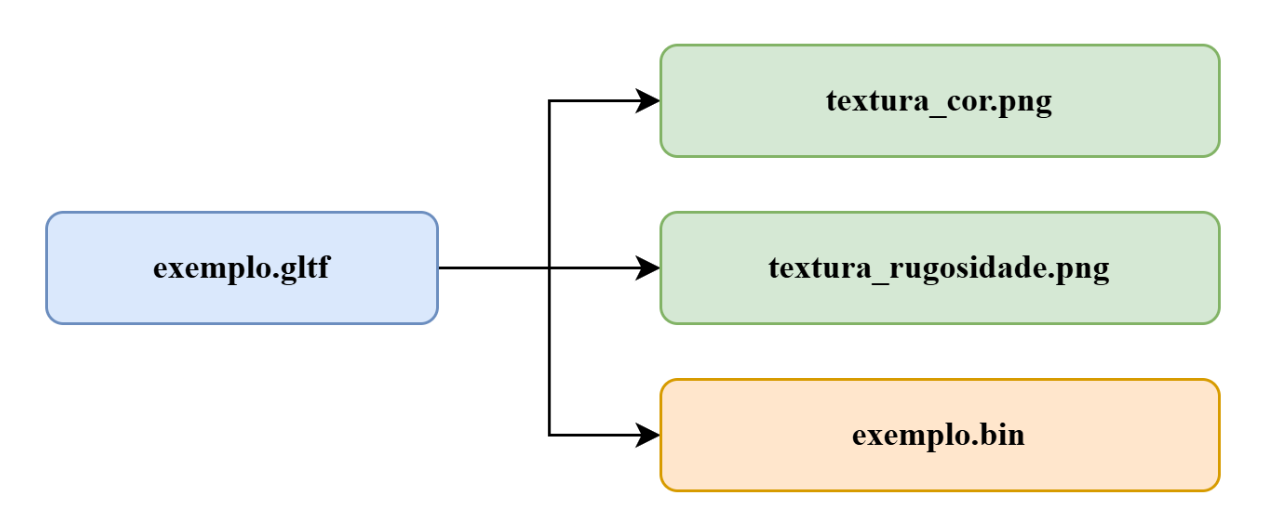
\includegraphics[width=0.8\textwidth]{figuras/estrutura-gltf.png}}
  \fonte{Autoria própria (2026).}
\end{figure}

\subsection{O contêiner GLB}

Alternativamente, o formato suporta o contêiner .glb, que consolida todos esses componentes em um único arquivo binário e utiliza uma estrutura de \textit{chunks} para facilitar o transporte e evitar múltiplas requisições de rede \cite{Khronos2021}.

O arquivo \gls{json} é o esqueleto que define a estrutura do binário impondo restrições rígidas para simplificar a implementação. Com isso, deve usar codificação \gls{utf8} sem conter a sequência de \textit{bytes} inicial; as chaves de objetos devem ser únicas e nomes de propriedades devem usar apenas caracteres \gls{ascii}. A organização interna do \gls{json} é feita através de \textit{arrays} de objetos, onde a comunicação entre os diferentes elementos ocorre obrigatoriamente através de índices. Nesse sentido, pode-se entender como referência à posição do objeto no \textit{array}. Os principais elementos descritos são \textit{scenes} e \textit{nodes} e eles definem a estrutura básica e a hierarquia da cena \cite{Khronos2021}.

Além dos elementos estruturais de nós e cenas, o arquivo \gls{json} do \gls{gltf} também define componentes que modulam a cena em sua totalidade, detalhando aspectos visuais e comportamentais dos objetos tridimensionais \cite{Khronos2021}:

\begin{alineas}
  \item As \textit{meshes} descrevem a geometria fundamental dos objetos através de
  primitivas de renderização, que definem se o ativo deve ser desenhado como
  pontos, linhas ou triângulos. Internamente, essas primitivas referenciam
  atributos de vértices, como a posição e os vetores normais, utilizando índices de
  \textit{accessors} que apontam para os dados brutos no arquivo binário;

  \item Os \textit{materials} especificam as propriedades ópticas dos modelos,
  incluindo mapeamentos de cor base, metalicidade, rugosidade e texturas de
  normais. Esses materiais definem como a luz reage à superfície e à profundidade
  da malha, influenciando diretamente a aparência visual do objeto;

  \item \textit{Animations} operam através de uma estrutura de canais e
  \textit{samplers}. Os canais definem o alvo da animação, como a translação,
  rotação ou escala de um nó, ou os pesos de um ponto de deformação. Os
  \textit{samplers}, por sua vez, gerenciam os dados de tempo e os valores
  correspondentes;

  \item As \textit{cameras} estabelecem as configurações de projeção necessárias
  para a visualização da cena pela aplicação.
\end{alineas}

Podemos entender melhor as divisões do arquivo \gls{json} na
Figura~\ref{fig:estrutura-json-gltf}.

\begin{figure}[htb]
  \centering
  \caption{\label{fig:estrutura-json-gltf}Divisões internas do arquivo JSON no formato glTF}
  \fbox{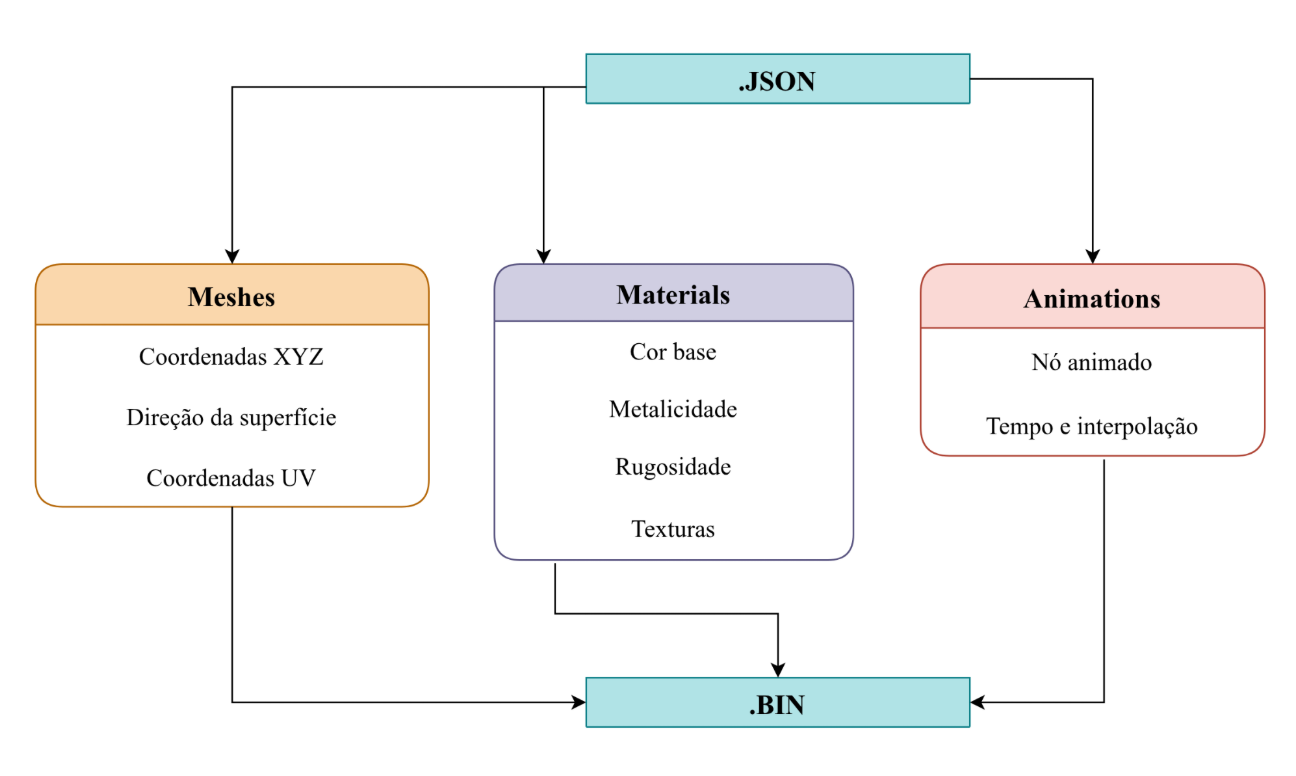
\includegraphics[width=0.8\textwidth]{figuras/estrutura-maior-gltf.png}}
  \fonte{Autoria própria (2026)}
\end{figure}

Uma funcionalidade crítica do \gls{json} é o referenciamento de recursos externos
por meio de \glspl{uri}, o que permite que as texturas e os dados binários residam
em arquivos separados. Para acessar e interpretar os dados brutos contidos no
arquivo binário, o \gls{gltf} utiliza uma estrutura de três camadas
interdependentes dentro do \gls{json}, garantindo a organização e a leitura
eficiente das informações \cite{Khronos2022}.

A primeira camada é composta pelos \textit{buffers}, que apontam para o recurso
binário completo e definem o seu tamanho total em \textit{bytes}. Em seguida, as
\textit{bufferViews} segmentam esse \textit{buffer} em fatias menores,
identificando quais partes pertencem especificamente aos dados de vértices, índices
ou animações. Por fim, os \textit{accessors} fornecem a interpretação tipada dos
dados dentro de uma \textit{bufferView}, definindo, por exemplo, que uma
determinada sequência de \textit{bytes} deve ser lida como um vetor de três números
flutuantes. Essa hierarquia permite que a aplicação decodifique a geometria e os
comportamentos do modelo de forma estruturada \cite{Khronos2022}.

A aplicação prática dessa hierarquia pode ser observada na
Figura~\ref{fig:gltf-buffers}, que ilustra a decomposição de um triângulo no plano
XY através das três camadas mencionadas. Na base da estrutura, o
\textit{geometryBuffer} representa o arquivo binário completo em uma sequência de
44 \textit{bytes} brutos. Essa unidade é segmentada pelas \textit{bufferViews}, que
recortam regiões específicas para os índices dos triângulos e para os atributos de
vértice. Por fim, os \textit{accessors} realizam a interpretação tipada desses
dados, convertendo os \textit{bytes} em valores compreensíveis para a aplicação,
como vetores de três números flutuantes que definem as coordenadas espaciais dos
vértices na origem e nos eixos correspondentes. Esse processo demonstra como o
formato \gls{gltf} organiza a geometria de forma otimizada, permitindo que dados
hexadecimais complexos sejam transformados em elementos visuais tridimensionais com
baixo custo de processamento.

\begin{figure}[htb]
  \centering
  \caption{\label{fig:gltf-buffers}Representação da hierarquia de camadas em um modelo}
  \fbox{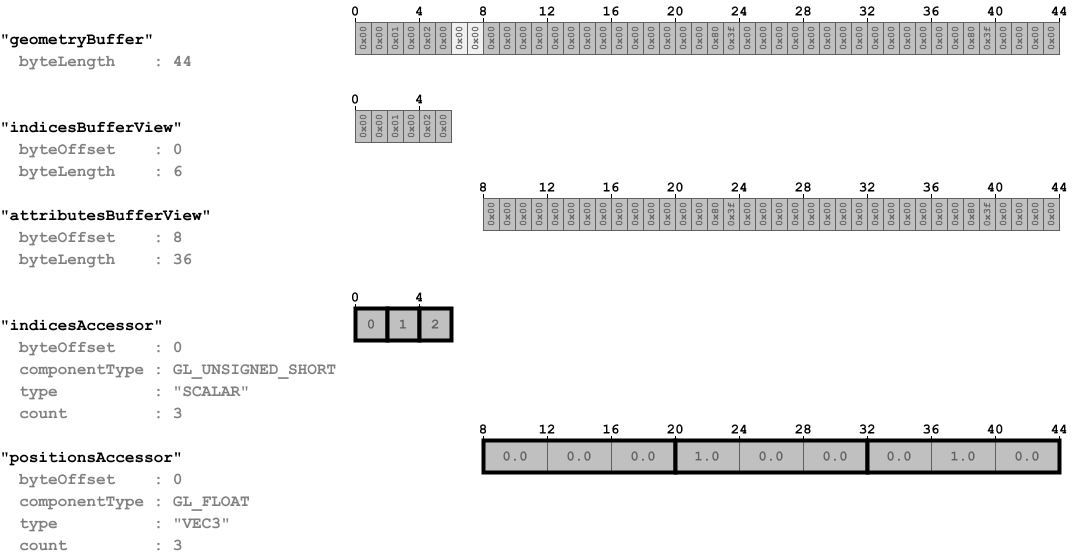
\includegraphics[width=0.8\textwidth]{figuras/gltfs-buffer.png}}
  \fonte{\citeonline{Khronos2022}}
\end{figure}

\subsection{Arquivos similares}
\label{sec:arquivos-similares}

Assim como o \gls{gltf} utiliza \textit{buffers} e \textit{bufferViews} para
organizar dados brutos em pedaços lógicos independentes, outros formatos de arquivo
possuem abordagens semelhantes. O \gls{tiff}, por exemplo, conforme especificado
pela \citeonline{Aldus1992}, é um formato de imagem rasterizada estruturado em
etiquetas, que descrevem e armazenam dados de imagem através de campos lógicos com
identificadores e valores. Sua criação garante independência e portabilidade, não
estando vinculado a processadores, sistemas operacionais ou \textit{hardware}
específicos, o que o torna possivelmente extensível ao método proposto neste
trabalho. A organização modular do \gls{tiff} é evidenciada pelo seu cabeçalho, que
aponta para um diretório de arquivos de imagem. Este diretório contém informações
cruciais sobre a imagem e, mais importante, os ponteiros, \textit{offsets} como
vistos no \gls{gltf}, para a localização real dos dados brutos no arquivo. O
formato suporta a segmentação da imagem em pedaços menores, permitindo que esses
segmentos sejam armazenados de forma fragmentada e acessados de maneira aleatória e
eficiente \cite{Aldus1992}.

De forma análoga, o formato \gls{wave} para áudio, conforme especificações
conjuntas da IBM Corporation e da Microsoft Corporation \cite{IBM1991}, organiza
seus dados brutos em segmentos lógicos independentes. O \gls{wave} adota uma
arquitetura etiquetada que promove um arquivo compatível. O arquivo é composto por
blocos, cada um com um identificador único e um campo indicando seu tamanho,
permitindo que aplicações ignorem blocos não reconhecidos. Para ser válido, um
arquivo \gls{wave} deve conter obrigatoriamente um bloco de formato, que define as
propriedades do áudio, e um bloco de dados, com as amostras binárias brutas. O
bloco de formato detalha parâmetros técnicos essenciais, como categoria do formato,
número de canais, taxa de amostragem e alinhamento de blocos.

\section{Trabalhos relacionados}

Esta seção apresenta uma análise de trabalhos relacionados que abordam o controle de versão e histórico de edição em contextos de imagens e modelos 3D.

\subsection{Controle de revisão não linear para imagens}

O trabalho desenvolvido por \citeonline{Chen2011} apresenta um sistema de controle
de versão para imagens digitais, que se diferencia dos métodos tradicionais ao
registrar as ações de edição do usuário em vez de armazenar o arquivo completo a
cada versão. Este enfoque visa otimizar o armazenamento e introduzir funcionalidades
avançadas de manipulação do histórico de edições.

O funcionamento do sistema baseia-se em duas estruturas primárias, o \gls{dag} e o
\gls{revg}. O \gls{dag} constitui o cerne do sistema, no qual cada nó representa uma
operação de edição, como pinceladas ou ajustes de cor, e as arestas estabelecem as
dependências temporais, espaciais e semânticas entre essas ações. Ações que afetam
diferentes partes da imagem são dispostas em caminhos paralelos, permitindo um
histórico de edição não linear. O \gls{revg}, por sua vez, oferece uma visualização
de múltiplas resoluções do \gls{dag}, utilizando miniaturas para representar o
progresso das edições e facilitar a navegação no histórico, a criação de
ramificações e a fusão de versões. Para o registro e reprodução das edições, o
sistema emprega um sistema de \textit{log}, que captura discretamente as ações do
usuário em \textit{softwares} como o GIMP, e um método capaz de reconstruir qualquer
estado da imagem a partir desses registros. Um filtro de importância visual também é
utilizado para agrupar nós do \gls{dag} no \gls{revg}, priorizando a relevância das
ações para uma interface mais limpa \cite{Chen2011}.

A Figura~\ref{fig:chen-dag} demonstra o uso da estrutura de grafos para armazenar as
edições na imagem. A partir de uma imagem original, são realizadas operações de
edição, como cópia, translação, deformação e ajustes de cor, gerando diferentes
revisões da imagem. Essas ações são organizadas na estrutura \gls{dag}, que
representa as dependências temporais, espaciais e semânticas entre as edições,
permitindo visualizar e gerenciar o histórico de modificações de forma não linear
\cite{Chen2011}.

\begin{figure}[htb]
  \centering
  \caption{\label{fig:chen-dag}Alterações em uma imagem de entrada}
  \fbox{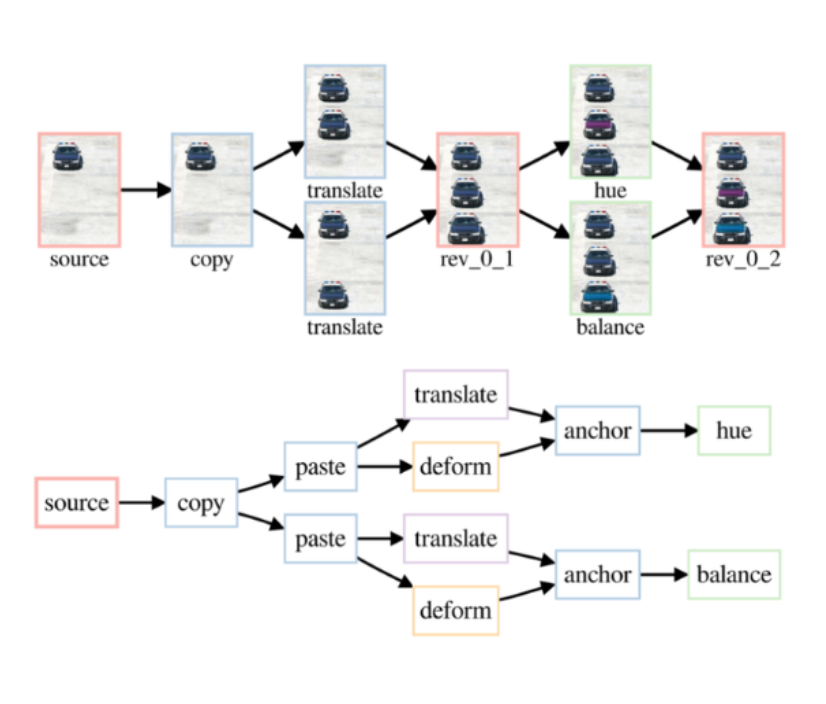
\includegraphics[width=0.8\textwidth]{figuras/chen-2011.png}}
  \fonte{\citeonline{Chen2011}}
\end{figure}

\subsection{\textit{Framework} de controle de revisão 3D}

\citeonline{Dobos2012} propõem um sistema de controle de versão para ativos 3D, com
foco em cenas massivas e edição colaborativa. Este sistema utiliza um banco de dados
\gls{nosql}, MongoDB, como repositório central. A cena 3D é desconstruída em um
Grafo de Cena, no qual componentes como malhas, materiais e câmeras são armazenados
como documentos binários individuais no formato \gls{bson}. O versionamento ocorre
no nível do documento, garantindo que apenas as partes alteradas da cena sejam
salvas em novas revisões, otimizando o uso de espaço.

O \textit{framework} opera através de duas interfaces principais: uma para o
usuário, que gerencia revisões e resolução de conflitos, e um cliente \textit{web}
somente leitura que utiliza \gls{webgl} para visualização remota. O método de
gerenciamento de revisões é estruturado por dois grafos, sendo o primeiro o Grafo de
Cena, que representa a estrutura lógica do modelo 3D, e o Histórico de Revisão, que
acompanha a evolução temporal do projeto, suportando ramificações e fusões. A
estrutura do histórico de revisões, ilustrada na Figura~\ref{fig:dobos-historico},
organiza o versionamento como um \gls{dag}, no qual cada nó representa uma revisão
com suas respectivas mudanças incrementais sobre o grafo de cena. A linha principal
de desenvolvimento evolui linearmente, enquanto ramificações permitem linhas de
desenvolvimento paralelas, que podem ser reintegradas através de operações de
\textit{merge}. Este modelo de versionamento, que armazena apenas as mudanças
incrementais dos nós do grafo de cena, reduz significativamente o custo de
armazenamento em comparação com sistemas tradicionais que tratam arquivos binários
3D como unidades atômicas. Para recuperar uma versão específica, o algoritmo
percorre o histórico de ancestrais, selecionando a versão mais recente de cada
objeto dentro da linhagem. No processo de fusão, uma ferramenta de comparação entre
objetos tridimensionais é empregada para identificar e visualizar conflitos
\cite{Dobos2012}.

\begin{figure}[htb]
  \centering
  \caption{\label{fig:dobos-historico}Estrutura do histórico de revisões e evolução do modelo}
  \fbox{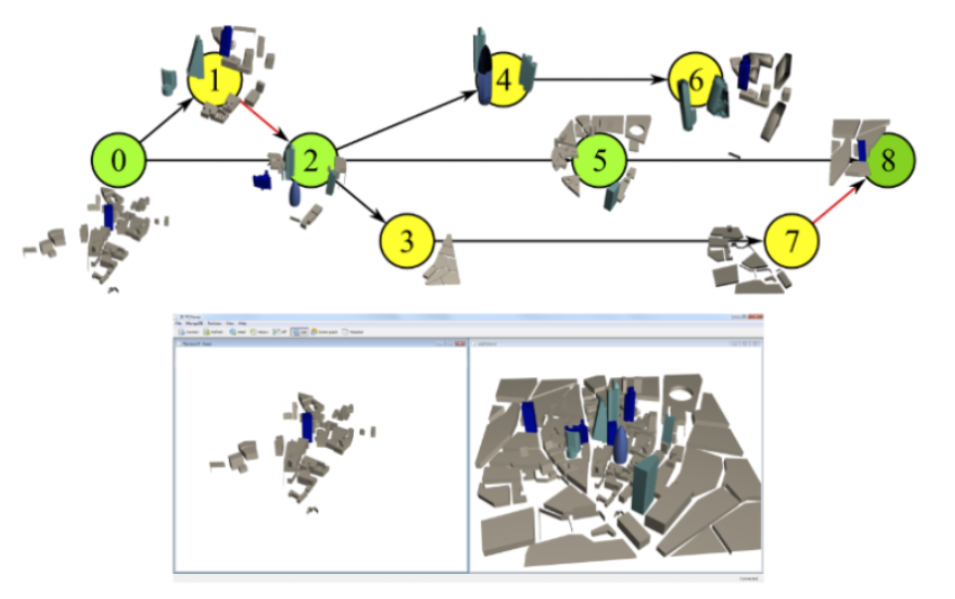
\includegraphics[width=0.8\textwidth]{figuras/dobos-2012.png}}
  \fonte{\citeonline{Dobos2012}}
\end{figure}

\subsection{Suporte a compressão delta em sistemas de arquivos}

\citeonline{MacDonald2000} propõe o \gls{xdfs}, um sistema de arquivos desenvolvido
para gerenciar de forma eficiente o armazenamento e o transporte de versões de
arquivos binários por meio de compressão delta, técnica que registra apenas as
diferenças entre duas versões de um arquivo em vez de armazenar cópias completas.

O sistema utiliza o algoritmo Xdelta, que emprega funções de impressão digital sobre
sequências de \textit{bytes} para identificar trechos correspondentes entre versões
e gerar um pacote contendo apenas as modificações. Para garantir que o tempo de
inserção de uma nova versão seja independente do tamanho total do histórico
armazenado, o \gls{xdfs} adota um mecanismo de transações baseado em banco de dados,
resolvendo um problema presente em sistemas anteriores, nos quais o arquivo de
histórico precisava ser reescrito integralmente a cada atualização.

O trabalho oferece duas estratégias complementares de armazenamento. A primeira
prioriza a velocidade de recuperação, garantindo que qualquer versão possa ser
reconstruída com a aplicação de no máximo um pacote de diferenças. A segunda
prioriza a economia de espaço, encadeando as diferenças em ordem inversa a partir da
versão mais recente. O sistema também foi projetado para eficiência na transmissão
de dados em rede, permitindo extrair diferenças entre quaisquer duas versões sem
reconstruí-las integralmente \cite{MacDonald2000}.

Apesar das vantagens em termos de desempenho no processamento de arquivos binários,
o \gls{xdfs} apresenta limitações relevantes. O custo de metadados gerado pelo banco
de dados interno pode superar o tamanho dos próprios dados comprimidos, e o processo
de criação de um novo histórico é significativamente mais lento do que em sistemas
de arquivos convencionais. Além disso, conforme discutido na
Seção~\ref{sec:arquivos-similares} deste trabalho, o sistema não lida adequadamente com
arquivos que possuem compressão interna, pois pequenas alterações no conteúdo
original resultam em mudanças massivas nos \textit{bytes} armazenados, anulando os
benefícios da abordagem diferencial \cite{MacDonald2000}.

\subsection{Análise comparativa dos trabalhos relacionados}

Os trabalhos apresentados nas seções anteriores abordam o versionamento de arquivos
sob perspectivas distintas, e esta seção traça um paralelo entre essas abordagens e
a proposta deste trabalho.

\citeonline{Dobos2012} adotam um banco de dados \gls{nosql} como repositório
central, exigindo a substituição do sistema de arquivos por uma infraestrutura
dedicada. O presente trabalho segue o caminho oposto, aproveitando as capacidades
nativas de sistemas de arquivos modernos para realizar o armazenamento diferencial
de forma transparente, sem dependências externas. Além disso, enquanto os autores
segmentam o modelo segundo sua estrutura lógica de cena, a abordagem aqui proposta
utiliza os segmentos internos definidos pelo próprio formato do arquivo como unidade
de versionamento.

\citeonline{MacDonald2000} propõe uma solução baseada em compressão delta que trata
qualquer binário como uma sequência opaca de \textit{bytes}, sendo agnóstica ao
formato do arquivo. A proposta deste trabalho difere em dois aspectos: em vez de
calcular diferenças \textit{byte} a \textit{byte}, utiliza funções de resumo
criptográfico para identificar segmentos inalterados, delegando ao sistema de
arquivos o compartilhamento físico desses blocos; e, ao segmentar o binário segundo
sua estrutura interna, garante que uma alteração localizada não produza mudanças em
cascata por todo o conteúdo.

\citeonline{Chen2011} versionam não os dados do arquivo, mas o registro das ações de
edição do usuário, o que exige integração direta com o \textit{software} de edição.
O presente trabalho atua em uma camada distinta, tendo como objeto de versionamento
os próprios \textit{bytes} resultantes da edição, tornando a abordagem compatível
com qualquer fluxo de trabalho de produção sem instrumentação adicional.

Em síntese, o que diferencia a proposta deste trabalho dos demais é a combinação
entre sensibilidade à estrutura interna do arquivo e o uso de mecanismos nativos do
sistema de arquivos, partindo do princípio de que arquivos binários com segmentação
interna bem definida são candidatos naturais ao versionamento eficiente por blocos.